\documentclass{article}
\usepackage{graphicx} % Required for inserting images
\usepackage{amsmath}
\usepackage[english, russian] {babel}
\usepackage[utf8]{inputenc}
\usepackage[T2A]{fontenc}
\usepackage{minted}
\usepackage{float}
\usepackage{amssymb}

\title{Теория вероятности и математическая статистика}
\author{silvia.lesnaia }


\begin{document}

\maketitle

\textbf{03.09.25}

\section{Глава 1 Условное распределение}


$(\Omega, \mathcal{F}, \mathbb{P}   )$ - $\Omega $ множество элементарных исходов,
$A\subset \Omega $ случайное событие 

$\mathcal{F} - \varsigma $ - алгебра событий: $(1)\Omega \in \mathcal{F},(2) A \in \mathcal{F}\Rightarrow $
$\Rightarrow \overline{A} \in \mathcal{F}; (3)\left\{ A_n\right\}_{i=1}^\infty  \in$
$\mathcal{F}\Rightarrow \bigcup _{n = 1}^{\infty} A_i \in \mathcal{F}$
$P:\mathcal{F}\rightarrow \left[0,1\right];$ т.е $P(A)$ - вероятность события A верхняя мера


(1)$P(A)\geq 0 \bigvee A \in \mathcal{F}, (2) P(\Omega) = 1$

(3) $P(\bigsqcup _{n = 1}^{\infty} A_i )= \sum_{n = 1}^{\infty} P(A_i) $

Определение: Случайная величина $\xi : \Omega \rightarrow \mathbb{R}, $ т.ч
$\bigvee x \in \mathbb{R}$ $\left\{w: \xi(w)<x \right\} \in \mathcal{F}$
$\xi_{-1}(b)  \in \mathcal{F}; b=(- \infty; x)$ 

утуттутутут
что то 



Определение: Случайный вектор это $\overline{\xi} = (\xi_1,\xi_2, \dots, \xi_n)$
где, $\xi_i$ случайная величина в $(\Omega, \mathcal{F}, \mathbb{P}); \Omega=\Omega_1* \dots *\Omega_n$
$\mathcal{F} -\varsigma $ алг

$\mathbb{P}$ - вероятностная мера

Рассмотрим $(\xi, z)$

Определение: Функция распределения

$F_{s,f} (x_i,y) = P\left\{w : \xi (w) < x ; \eta (w) < y \right\} $

\begin{figure} [H]
    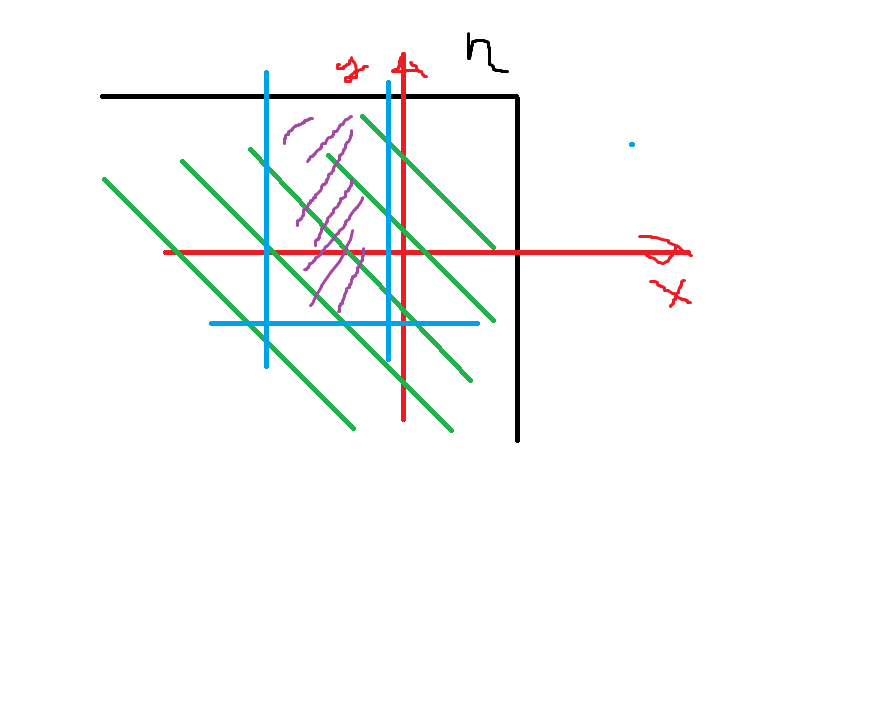
\includegraphics[width=0.50\linewidth]{Без имени.png}
\end{figure}

Свойства:

(1)

(2)



\end{document}